
\documentclass[../master.tex]{subfiles}

\begin{document}

\section{Design}
One of our most important design goals is to make the program as conceptually sane and maintainable as possible (see \hyperref[sec:Goal3]{goal 3}). Moreover, by having to build on DIKUArcade and meeting all of the given requirements (see \hyperref[sec:Goal1]{goal 1}), it has had a great impact on our design decisions.

\subsection{Design decisions}
In the following first table we have created a responsibility table, where we describe some concepts of our design we need to implement for \textit{Space Taxi}.
\renewcommand{\arraystretch}{1.5}
\begin{table}[h]
	\centering
	\label{my-label}
	\begin{tabular}{|l||l|}
		\hline
		\multicolumn{2}{|c|}{\textbf{Responsibility}}                                     \\ \hline
		\multicolumn{1}{|l||}{\textbf{Responsibility description}} & \multicolumn{1}{l|}{\textbf{Concept name}} \\ \hline
		Load level to simple data structure.         & Loader                                     \\ \hline
		Generate level entities.                     & levelParser                                \\ \hline
		Container which hold level entities.         & Level                                      \\ \hline
		Player entity.                               & Taxi                                       \\ \hline
		Obstacles where a taxi can land.             & Platform                                   \\ \hline
		Non-moving entities.                         & Obstacle                                   \\ \hline
	\end{tabular}
\end{table}

\newpage

In the following table we will deduct the associations between our concepts of the design. I.e. how our concepts are related.
\renewcommand{\arraystretch}{1.5}
\begin{table}[h]
	\centering
	\begin{tabular}{|p{3.5cm}||p{5cm}|p{4cm}|}
		\hline
		\multicolumn{3}{|c|}{\textbf{Responsibility}}                                                                                                                                                 \\ \hline
		\multicolumn{1}{|c||}{\textbf{\begin{tabular}[c]{@{}c@{}}Concept Pair\end{tabular}}} & \multicolumn{1}{c|}{\textbf{Association descriptions}} & \multicolumn{1}{c|}{\textbf{Associate name}} \\ \hline
		levelParser $\leftrightarrow$ Loader & LP using data structure from Loader to create level. & makeMap, getTaxiPosition, makePlatforms, makeObstacles \\ \hline
		Level $\leftrightarrow$ levelParser  & Level get object from LP. &  getLevel \\ \hline
		Taxi $\leftrightarrow$ Level  & Level knows about taxi.   &  getTaxiPosition  \\ \hline
		Platform $\leftrightarrow$ Level  &  Platform is part of a level.  & platforms (list of platforms) \\ \hline
		Platform $\leftrightarrow$ Taxi   &  Platform knows about taxi.    &  isLanding, Landing          \\ \hline
		Obstacle $\leftrightarrow$ Level  &  Object is part of a level.    &  obstacles (list of obstacles) \\ \hline
		Obstacle $\leftrightarrow$ Taxi   &  Taxi collide with an object.  &  collideWith             \\ \hline
	\end{tabular}
\end{table}

\newpage

In the tables before, we have identified the main responsibilities and their associations in our design of the game. Therefore, we will now consider what kinds of attributes our concepts in our game requires.
\begin{table}[H]
	\centering
	\begin{tabular}{|c||l|l|}
		\hline
		\multicolumn{3}{|c|}{\textbf{Responsibility}}                                                                                                                                                       \\ \hline
		\textbf{Concept} 	     & \textbf{Attributes}    & \textbf{Attribute Description} 		    \\ \hline
		\multirow{1}{*}{Loader}  & Level                  & list of strings						    \\ \cline{2-3}
		\hlineB{2}
		
		\multirow{6}{*}{LP}      & Height  			& Number of rows in the map					    \\ \cline{2-3}
		& Width			& Number of chars in a row 						\\
		\cline{2-3}
		& level     	    & List of strings given from Loader             \\ \cline{2-3}
		& map	 	   		& Sublist of level which contain the gamemap    \\ \cline{2-3}
		& images  			& Dictionary of keys and correspondend image    \\ \cline{2-3}				
		&	name			& Level name									\\ \cline{2-3}
		& 	xscale			& ratio on the x-axis of number of elements		\\ \cline{2-3}
		& 	yscale			& ratio on the y-axis of number of elements		\\ \cline{2-3}
		& errorMessage 	& Internal error handler						\\ \cline{2-3}
		\hlineB{2}
		
		\multirow{5}{*}{Taxi}    & position        & Position of the player	  					    \\ \cline{2-3}
		& image           & Graphical representation of the player	        \\ \cline{2-3}
		& direction  	   & tracker for direction						    \\ \cline{2-3}
		& hasCustomer     & Boolean value corresponding to the name	    \\ \cline{2-3}
		& shape  	       & physical parameters of the taxi			    \\ \cline{2-3}
		\hlineB{2}
	\end{tabular}
\end{table}

\subsection{The overall structure of the game}
\textbf{Game}
\begin{itemize}
	\item[] Game is a singleton class, around which the entire game evolves.\\
	This class is a non-terminal method GameLoop, which render the game screen through the different states and entities. This class also maintains the statemachine and the eventbus (SpaceTaxiBus) which send the keyboard events to statemachine.
\end{itemize}
\textbf{SpaceTaxiBus}
\begin{itemize}
	\item[] A singleton class, that is a wrapper for the DIKUArcade.EventBus the solo purpose of this is to get a static eventbus to be called from anywhere in the program.
\end{itemize}
\textbf{StateMachine}
\begin{itemize}
	\item[] A singleton class, that handle the state switch and direct the events to the active state.
\end{itemize}

\textbf{States}
\begin{itemize}
	\item [] \textbf{MainMenu} -- Initiate state where the player can enter a new game or quit. 
	\item [] \textbf{NextLevel} -- This state will handles the state where the ship teleport to a new level, that has the new environment, background, objects, obstacles and platforms.
	\item [] \textbf{GamePaused} -- This state pauses the game momentarily, where the player should be able to quit the game.
	\item [] \textbf{Quit} -- This state will quit the game.\\
\end{itemize}

\textbf{LevelBuilder}
\begin{itemize}
	\item[] \textbf{IFetcher} -- will be an interface the loader will use to comply with some expectations of the output.
	\item[] \textbf{IParser} -- will be an interface the parser will use to comply with some expectations of the output.
	\item[] \textbf{Level} -- will handle an active level.
	\item[] \textbf{LevelParser} -- LevelParer is an iparser, an implementation as given a list of strings making all level entities, which level can accept.
	\item[] \textbf{Loader} -- is an IFetcher implementation, it takes a filepath and returns a list of strings that the file constitutes and removes any blank lines.\\
\end{itemize}
\begin{figure}[H]
	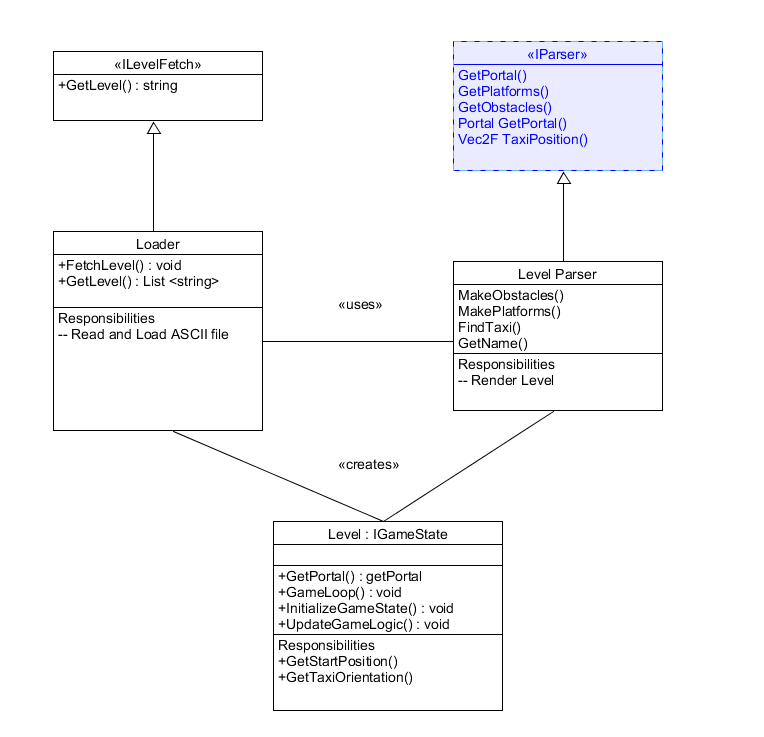
\includegraphics[width=\textwidth]{UML}
	\caption{UML representation of our Loader and Level implementation}
\end{figure}
\textbf{SpaceTaxiEntities}
\begin{itemize}
	\item[] \textbf{ICollision} -- is an interface that all the SpaceTaxiEntities will implement, except the player. Uses a boolean CollidWith.
	\item[] \textbf{Customers} -- implements the interface ICollision that will use this, so when the player collides with the customer, the customer should disappear. It will handle them in general, but it will get all data for all the customers.
	\item[] \textbf{Obstacles} -- implements the interface ICollision that will use this, when the player collides with an obstacle, it should explode.
	\item[] \textbf{Platforms} -- implements the interface ICollision, that will use this, when the player gets close to the platform it should land.
	\item[] \textbf{Player} -- Everything there is about the player will be handled in here. Orientation, images, animations, player speed etc.
	\item[] \textbf{Portal} -- will be the port that will teleport the player to the next level. It will uses collision detection to detect when the player collides with the portal area, it should teleport the player to the new area.\\
\end{itemize}

\textbf{Movement}
\begin{itemize}
	\item[] \textbf{IMovement} -- is an movement interface that will have a method void Move.
	\item[] \textbf{OnPlatform} -- will be used to track movement near a platform. It will also make sure that when the player-ship is on the platform, it should not fall off the platform, which means it turns off gravity temporarily.
	\item[] \textbf{TrivialMovement} -- All the physics in the game will be handled in here.\\
\end{itemize}

\textbf{GameConstants}
\begin{itemize}
	\item[] This static class handles all constants in the game. For example, player speed, physics, screen size, explosion duration, and the game timers.
\end{itemize}

\subsection{How well did we follow the SOLID principles?}
The SOLID-Principles, which stands for:
\begin{enumerate}
	\item Single responsibility (SRP)
	\item Open-closed (OCP)
	\item Liskov substitution (LSP)
	\item Interface segregation (ISP)
	\item Dependency inversion (DIP)
\end{enumerate}

In terms of the SOLID-Principles we have chosen to represent each of them the following way, so we can describe how well we have followed them:\\

\noindent\textbf{Single responsibility:}\\
The single responsibility principle is about that every class, function, variable should define a single responsibility. That means it has only one reason to change. If you change anything in that class, it will effect only one particular behavior of the software.\\

\noindent So in terms of SRP we have for example the player-class. In this player class, everything there is about the player is inside this class. The player-movement, the physics affecting the player, the player orientation, thrusters, images. And every variable in this class is for one thing only. We have: the GravityDirection variable is only used to make gravity, the ThrusterDirection concerns only about the thrusters and so on. Other examples could be our Obstacles class, Platforms class and Portal class, which only concern about the obstacles, the platform and the portal (which changes level by the player ``colliding`` with it).\\

\noindent\textbf{Open-closed:}\\
The open-closed principle concerns that software entities (classes, modules, functions, etc.) should be open for extension, but closed for modification. Such that an entity can allow its behavior to be extended without modifying its source code. This can be achieved with inheritance. You don’t have to touch the class you want to extend if you create a subclass of it.\\

\noindent To cover the open-closed principle we for example use inheritance a lot in our program. We have e.g. an interface ``ICollision`` which will handle the different types of collisions. As colliding with a platform it should have one action, than colliding with a wall. We use this Interface in the separate classes: Customer, Obstacles, Platforms and Portal, which also inheritances from another class called Entity, which handles entities.\\

\noindent\textbf{Liskov substitution:}\\
The Liskov substitution principle concerns objects in a program, that should be replaceable with instances of their subtypes without altering the correctness of that program. It can be though of an extension of the Open-Closed principle.  
\\

\noindent In our game we use this with the parser and the fetcher. The constraints on the substitute of the class are fairly weak, since we only demand that the output has a certain type. But nevertheless we could substitute the loader with one which load the levels of github, or some other place.
\\

\noindent\textbf{Interface segregation:}\\
The interface segregation principle concerns that no client should be forced to depend on methods it does not use. That means classes should be as specialized as possible. You do not want any ``god`` classes that contain the whole application logic.\\

\noindent In our game we for example have the game elements: Customer, Obstacles, Platforms, Portals and the player, that all should have the feature ``collision''. Some will use this feature different than the others. That means, for example when the player-ship collides with an obstacle it should explode, but if the ship collides with a portal it should teleport the player to the next game level. So instead of we have one class which performs all the actions, we have created an Interface and 5 different classes, one for each event type. We have therefore also made a ICollision interface so the client will not be forced to depend on methods it does not use. And we have our 6 classes: Customer, Obstacles, Platforms, Portals and the player, where Customer, Obstacles, Platforms, Portals uses the interface ICollision to make their own collision action.\\

\noindent\textbf{Dependency inversion:}\\
The dependency inversion is about that high-level modules should not depend on low-level modules: both should depend on abstractions. To create specific behavior you can use techniques like inheritance or interfaces.\\

\noindent We have for example use this in the way we load our game level. The concrete way in which the implementation of our interface Ifetcher operates is not dominant of how Iparser reads it. The interface Iparser implementation has only the requirement that the output is the same structure (i.e. List<string>), besides that Ifetch of course also expects the level text-file to have a specific setup. As well as that level uses the Iparser interface and gets some output, but how it is found and made does not matter to the level class.\\

\noindent\textbf{Conclusion}\\
Overall, we think we have done the best to follow the SOLID Principles, but as we know, where are always things that can be improved. We haven't used some of the SOLID Principles as much as the others. That could for example be the Liskov substition principle. In our code, we have not used this principle as much, because we have chosen to implement our code leaning more heavily on the simpler, Open-Closed principle.

\end{document}
